% Template for PLoS
% Version 1.0 January 2009
%
% To compile to pdf, run:
% latex plos.template
% bibtex plos.template
% latex plos.template
% latex plos.template
% dvipdf plos.template

\documentclass[10pt]{article}

% amsmath package, useful for mathematical formulas
\usepackage{amsmath}
% amssymb package, useful for mathematical symbols
\usepackage{amssymb}

% graphicx package, useful for including eps and pdf graphics
% include graphics with the command \includegraphics
\usepackage{graphicx}

\usepackage{bussproofs}

% cite package, to clean up citations in the main text. Do not remove.
\usepackage{cite}

\usepackage{color} 

% Use doublespacing - comment out for single spacing
%\usepackage{setspace} 
%\doublespacing

% Text layout
\topmargin 0.0cm
\oddsidemargin 0.5cm
\evensidemargin 0.5cm
\textwidth 16cm 
\textheight 21cm

% Bold the 'Figure #' in the caption and separate it with a period
% Captions will be left justified
\usepackage[labelfont=bf,labelsep=period,justification=raggedright]{caption}

% xy-pic for diagrams
\usepackage[all]{xy}
% subcaption
\usepackage{subcaption}
% hyperref
\usepackage{hyperref}
% color table cells http://goo.gl/ZmpJv
\usepackage[table]{xcolor}
%rotate text in table http://goo.gl/Lb4Zd
\usepackage{rotating}

\usepackage{crs}
% Use the PLoS provided bibtex style
\bibliographystyle{plos2009}

% Remove brackets from numbering in List of References
\makeatletter
\renewcommand{\@biblabel}[1]{\quad#1.}
\makeatother


% Leave date blank
\date{}

\pagestyle{myheadings}
%% ** EDIT HERE **


%% ** EDIT HERE **
%% PLEASE INCLUDE ALL MACROS BELOW

%% END MACROS SECTION

\begin{document}

% Title must be 150 characters or less
\begin{flushleft}
{\Large
\textbf{Title}
}
% Insert Author names, affiliations and corresponding author email.
\\
Author1$^{1}$, 
Author2$^{2}$, 
Author3$^{3,\ast}$
\\
\bf{1} Author1 Dept/Program/Center, Institution Name, City, State, Country
\\
\bf{2} Author2 Dept/Program/Center, Institution Name, City, State, Country
\\
\bf{3} Author3 Dept/Program/Center, Institution Name, City, State, Country
\\
$\ast$ E-mail: Corresponding author@institute.edu
\end{flushleft}

% Please keep the abstract between 250 and 300 words
\section*{Abstract}

% Please keep the Author Summary between 150 and 200 words
% Use first person. PLoS ONE authors please skip this step. 
% Author Summary not valid for PLoS ONE submissions.   
\section*{Author Summary}

\section*{Introduction}
Evolution is arguably the most fundamental organizing concept in biology. In order to understand biological systems, it will be necessary to address the question: What are the necessary enabling conditions that make biological evolution possible? The synthesis of some potential answers to this question may clarify a path toward defining a sufficient collection of preconditions for evolutionary processes to take flight.

Here we argue that one such necessary precondition for evolution is what we refer to as \emph{functional closure}. In order to define this term and its context, we begin with a diagrammatic model of a prototypical biochemical reaction network that has been claimed to possess this property. We then ask: Is there a formal language capable of expressing this property? A brief detour is necessary to motivate this question. In computer science, there is a property of languages called \emph{expressive power} that is used both heuristically and formally to rank order models of computation, programming languages, and their associated logics with respect to one another and with respect to so-called \emph{natural language}. Roughly speaking, an increased level of expressive power of a language correlates with its ability to express more complex or sophisticated ideas. One might ask why it is not always desirable to work within the extant language containing the highest possible expressive power. One reason to consider less expressive languages at all is that important questions about them can be answered algorithmically with appropriate computer hardware and software in a practical amount of time and memory, whereas the same questions posed of languages with more expressive power are known not to be able to be answered by such means.

In this light, we can refine the question, "Is there a formal language capable of expressing this property?" by adjoining the follow-up question, "If so, what is the language of minimal expressive power capable of expressing the functional closure property?" We begin to address the first question taking an historically motivated approach by attempting to interpret this diagram in terms of an abstract algebraic language called category theory. Unfortunately, the prototypical diagram violates a fundamental assumption of this language precisely because the diagram expresses the functional closure property. However, we find that this diagram, and indeed the functional closure property in general, can be interpreted in terms of a standard model of computation called (untyped or type-free) lambda calculus. We find that the interpretation of functional closure in terms of category theory can be recovered, albeit it in a form that looks quite different, via one typical category theoretic semantics for the untyped lambda calculus.

Although the untyped lambda calculus and its associated category theoretic semantics are capable of expressing the functional closure property, this method has at least two problems. One is that the untyped lambda calculus is a relatively expressive language capable of implementing general recursion. The second is that the untyped lambda calculus is capable of expressing functional closure in a trivial way via something as simple as an identity function. A simple solution might seem to pass to the simply typed lambda calculus, of which the untyped lambda calculus has been argued to be a special case. However, as a result of the analogous category theoretic semantics for the simply typed lambda calculus, doing so brings us back to the original category theoretic interpretation of the diagram expressing the functional closure property that we demonstrated to be in type-theoretic error.

This circularity seems to suggest that in order to address the second question regarding minimal expressive power necessary to express functional closure it may be necessary to take into account expressions of functional closure that may be possible to construct in various extensions of the simply typed lambda calculus (some of these may be found on the seven additional vertices of Barendregt's lambda cube). We discuss these issues with respect to the goal of identifying a language of minimal expressive power capable of representing the functional closure property or relevant approximations thereof.

% Results and Discussion can be combined.
\section*{Functional closure in biological terms}
\subsection*{Functional closure as an invariant property of evolvable systems}

In this section, we will attempt to explain the functional closure property in category theoretic terms. We will describe this property in the setting of a cartesian closed category (see Materials and Methods). Cartesian closed categories provide mathematical semantics for the simply typed lambda calculus \cite{Barendregt1985}. We will therefore sometimes refer to this setting as being ``typed''. This terminology is used to contrast the description in this section in terms of a cartesian closed category, which could be given equally well in terms of simply typed lambda calculus, with that in the next section in terms of the untyped lambda calculus. The abstract components have been related to biological ones in the previous section. The biological property from which Rosen derived his diagram expressing the functional closure concept is metabolism regarded in the manner described above and as depicted in Figure \ref{fig:metabolicstringdiag}. A metabolic mapping in an evolvable system $\mathcal{E}$ can be thought of as a morphism between two objects in $\mathcal{E}$, the latter now regarded as an abstract algebraic category:
\begin{align*}
f \colon A &\longrightarrow B\\
a &\longmapsto f(a)=b
\end{align*}

In category theory, we can imagine the abstract objects and morphisms as specializing to a particular type of algebraic structure and, thus, as a first approximation we can think of both objects as (cartesian product) sets, where $A$ represents a configuration of input substrates and $B$ likewise for metabolite products of metabolic transformations such as $f$. This abstraction of some aspects of an evolvable system could be further developed by substituting more highly structured objects than sets that meet intuitive and otherwise empirically suggested features of evolvable systems. We can consider all such \emph{metabolisms} together as the set of all the different morphisms between these objects referred to, if such an object exists at all, as the \emph{internal} exponential object $B^A$ \footnote{see Materials and Methods for the precise definition of exponetial object} or the \emph{external} hom-set $Mor_{\mathcal{E}}(A,B)$.

The apparently finite nature of evolvable systems, imposes several constraints regarding the maintenance of sufficient concentrations of the components that constitute it. As enzymes necessary for metabolism decay, they must be regenerated, from the metabolic products, or the system comprised of them will disintegrate. In addition, fluctuations in the substrates $A$ have to be corrected by the differential availability and performance of the overall metabolic morphism $f$. Hence, there must be a collection of morphisms from $B$ to $B^A$, one of which can be identified with the information required to \emph{regenerate} the enzymes necessary for core metabolic processes:
\begin{align*}
g \colon B &\longrightarrow B^A\\
b &\longmapsto g(b)=f
\end{align*}
This \emph{regeneration} system itself represented by $g \in B^{A^B}$ is also assumed to have a finite lifetime and thus requires a form of \emph{meta-regeneration} by some other system:
\begin{align*}
h \colon B^A & \longrightarrow B^{A^B}\\
f & \longmapsto h(f)=g.
\end{align*}	
In the biological metaphor commonly associated to this abstract construction, this \emph{meta-regeneration} system is associated either to the maintenance of some degree of structural invariance in the topology of the combined gene regulatory and metabolic interaction networks underlying an organism. In this light, this process may be associated to the DNA replication and reproduction process. In any case, the argument proliferating hierarchical levels of organization necessary to strive toward functional closure may be continued \emph{ad infinitum} (i.e. the next step would be to ask for the origin of $h$ and to posit the existence of another higher-order morphism that takes $g$ as input and produces $h$, see Figure \ref{fig:hom}b). 

From a biological perspective, systems of the form described may be able to avoid such an infinite regress by achieving a form of \emph{functional closure} in which, for example, we can materially identify a metabolic product $B$ with a replication function $h$ or perhaps even with the entire set of replication functions $B^{A^B{^B{^A}}}$. If we take the former case then we have introduced a problem that cannot be dealt with given the definition of a category because of the fundamental typing distinction therein between objects and morphisms. Although we might be able to associate an element or point of the object or type $B$ with $h \in B^{A^B{^B{^A}}}$, we sustain a typing error if we attempt to express the fact that these are materially equivalent because $h \colon 1 \rightarrow B$ is of type $B$ while $h \colon B^A \rightarrow B^{A^B}$ is of type $B^{A^B{^B{^A}}}$. Thus we would attempt to state $h:B = h:B^{A^B{^B{^A}}}$, but this is impossible to do, at least naively, within category theory as it produces a type error due to the fact that equations are only allowed between elements (respectively paths) with the same type (respectively with the same domain and codomain) Figure \ref{fig:hom}a. The other option is to avoid attempting to identify such elements and attempt to simply identify objects themselves. In this sense, we would attempt to express closure internally as $B \cong B^{A^B{^B{^A}}}$ or externally as $Mor_{\mathcal{E}}(1,B) \cong Mor_{\mathcal{E}}(B^A,B^{A^B})$. This approach could be considered to solve the typing issue since we could more explicitly state that $B \colon Set \cong B^{A^B{^B{^A}}} \colon Set$ or more generally for any category $B \colon Ob(\mathcal{E}) \cong B^{A^B{^B{^A}}} \colon Ob(\mathcal{E})$. However, we have now implied something stronger and less intuitive about the biological meaning of functional closure by stating that the set of metabolites is somehow isomorphic to the set of \emph{all possible} replication morphisms. Moreover, if such a relationship were to be satisfied, it could only be satisfied by the most trivial case in the category of sets $A = \{*\} = B$ so that $|B|=1=|B^{A^B{^B{^A}}}|$.

We have not yet attempted to make explicit how it might be possible to perform the identification between an element of type $B$ and another of type $B^{A^B{^B{^A}}}$ as expressed in Figure \ref{fig:hom}c. The original argument describing functional closure in a sense settles for stating something weaker than what we have already suggested is impossible to do directly within category theory (i.e. to state for some $h$, $h:B = h:B^{A^B{^B{^A}}}$). The most important feature of this argument is the concept of an evaluation map (see Materials and Methods) or morphism, which is intrinsic to the definition of exponential objects and thus evaluation maps exist in categories, like the primary example of the category of $\mathbf{Sets}$ we have considered thus far, having exponential objects. Given a category with products and exponentials, the evaluation map can be curried (i.e. in this case a function of two variables that returns a value can be converted to a function of one variable that returns a function) in the following manner
\begin{prooftree}
				\AxiomC{$B^{A} \times A \xrightarrow[]{ev} B$}
				\UnaryInfC{$A \xrightarrow[]{\hat{ev}} B^{B^A}$}
\end{prooftree}
where the maps $\hat{ev}$ are defined pointwise as
\begin{align*}
\hat{ev}(a) \equiv ev_a \colon B^A &\longrightarrow B,\\
f &\longmapsto ev(f,a) = f(a).
\end{align*}
This construction can be applied analogously at the next level regarding the evaluation of functions of the type $B^{A^B}$, by applying them to arguments of type $B$, to functions of the type $B^A$. The currying of the evaluation map is given by
\begin{prooftree}
				\AxiomC{$B^{A^B} \times B \xrightarrow[]{ev} B^A$}
				\UnaryInfC{$B \xrightarrow[]{\hat{ev}} B^{A^{B^{A^B}}}$}
\end{prooftree}
where the maps $\hat{ev}$ are defined pointwise as
\begin{align*}
\hat{ev}(b) \equiv ev_b \colon B^{A^B} &\longrightarrow B^A,\\
g &\longmapsto ev(g,b) = g(b).
\end{align*}
Although the continuation of the functional closure argument may also be applied in the first case of $ev_a$, we will apply it to the next level involving $ev_b$ to maintain the intuitive property that the metabolic substrate configuration represented by $A$ also represents material being extracted from the environment while functional closure is assumed to be achieved internal to the metabolic network (represented by $f$) and the regulatory apparatus (represented by $g$ and $h$) layered on top of it despite the material connection via $A$ to the environment.

We first consider the preimages of the evaluation morphisms as
\begin{align*}
\hat{ev}^{*}(b) \equiv ev^{*}_b \colon B^A &\longrightarrow B^{A^B},\\
f &\longmapsto g |g(b)=f.
\end{align*}
If, in this case, the evaluation morphism can be shown to have an inverse (i.e. $\hat{ev}^{*} \circ \hat{ev} = 1_A$ and $\hat{ev} \circ \hat{ev}^{*}= 1_{B^{B^A}}$) for some potentially restricted domain of definition of $\hat{ev}$ then the inverse morphism can also be defined pointwise as 
\begin{align*}
\hat{ev}^{-1}(b) \equiv ev^{-1}_b \colon B^A &\longrightarrow B^{A^B},\\
f &\longmapsto g | g(b) = f.
\end{align*}
In this sense, if there is a unique $g$ satisfying $g(b)=f$ for each combination of $b$ and $f$ in the restricted domains of definition then $b$ and $f$ can be viewed as determining $g$. This relieves what otherwise appears to be the necessity of positing the existence of an $h$ to answer the question of the origin of $g$. This is the weaker statement that is supported by this argument as compared to the stronger version, which could ostensibly be expressed as $b:B = h:B^{A^{B^{B^A}}}$.

\begin{figure}
\begin{center}
\noindent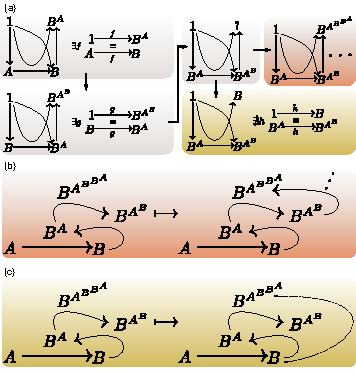
\includegraphics[width=0.75\columnwidth]{fig/mrcatclosure.pdf}
%\noindent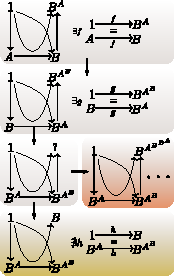
\includegraphics[width=0.24\columnwidth]{fig/mrcatprob.pdf}
\end{center}
\caption{Rosen's diagram attempting a depiction of functional closure in a cartesian closed category. (a) The top-left panel shows the identification of morphisms with domain $A$ and codomain $B$ with elements of the exponential object $B^A$. The bottom-left panel shows the analogous relationship between morphisms with domain $B$ and codomain $B^A$ and the exponential object $B^{A^B}$. On the right, two alternatives are shown in the last step. Either one can (b) continue on the path leading to infinite regress or (c) take the path leading to immediate closure.}
\label{fig:hom}
\end{figure}

\subsection*{Functional closure expressed in a type-free setting}
This argument describing functional closure so far suggests constraints by which we may be able to \emph{determine} some $h$ via $b$ (and also $f$), but so long as the ultimate goal is to state that for some $b$, $b:B = h:B^{A^B{^B{^A}}}$, it appears that it cannot be done in an obvious way in category theoretic terms. This is a result of the typing discipline inherent to the category theoretic description used thus far. We will ultimately find that we can re-express a stronger form of the functional closure in category theoretic terms, but in a manner that it is not obvious how to define directly within category theory. We thus first re-consider the expression of functional closure in terms of another language, the lambda calculus, which has both type-free and varying degrees of typed forms \cite{Barendregt1985} before returning to the so-called categorical semantics that enable the re-expression of this stronger form of functional closure in category theoretic terms.

If we reconsider the discussion in the previous section without regard for any typing discipline, we can summarize the proliferation of levels of organization up through the first three discussed in the following system of equations
\begin{align*}
f(a)&=b,\\
g(b)&=f,\\
h(f)&=g.
\end{align*}
It is trivial to express the functional closure property so long as we are able to disregard any typing discipline by identifying $h$ with $b$. In this case we can express functional closure as
\begin{align*}
f(a)&=b,\\
g(b)&=f,\\
b(f)&=g.
\end{align*}
Again, it is clear that in the typed setting this is not possible. In the typed setting we worked within the language of a cartesian closed category, which, as mentioned, provides mathematical semantics for the simply typed lambda calculus. Therefore, we may ask which language has sufficient expressive power to be able to state the functional closure property. We have just noted that the functional closure property can be directly expressed if we remove the typing constraint. This involves passing from the simply typed to the type-free lambda calculus. We will explain the syntax of the type-free lambda calculus and then, by analogy to the fact that cartesian closed categories provide semantics for the simply-typed lambda calculus, we will ask: Which mathematical structure is capable of providing mathematical semantics for the type-free lambda calculus?

In the Materials and Methods section, we provide a description of the syntax of the simply typed $lambda$-calculus and its semantics in terms of cartesian closed categories that was used in developing the model of functional closure in terms of a cartesian closed category. We have suggested that in order to be able to obtain a strong notion of equivalence between an object and a morphism, we need a language with at least some of the expressive capability of the type-free $\lambda$-calculus. We will therefore develop the analogous constructions of syntax and corresponding categorical semantics for the type-free lambda calculus.

\subsubsection*{The type-free lambda calculus and its categorical semantics}
The type-free lambda calculus can be seen as a special case of the simply-typed lambda calculus in which the set of basic types is restricted to contain only a single type. With the typing constraint imposed by having multiple types removed, it should be possible to perform self-application as in the term $\lambda x. xx$. If the second occurence of $x$ in this term has type $D$ and the whole term $xx$ has type $D$ then the first occurrence of $x$ in the term $xx$ must be construable as having type $[D \rightarrow D]$. A presentation of the type-free theory, $\mathbb{T}$, can then be given in a manner analogous to that of the simply typed lambda calculus:
\begin{enumerate}
\item{Types:}
\begin{align*}
&\mbox{one basic type: } D\\
\end{align*}
\item{Terms:}
\begin{align*}
&\mbox{variables: } x,y,z, \ldots \colon D\\
&\mbox{constants: } i \colon [D \rightarrow D] \rightarrow D,\,\, r \colon D \rightarrow [D \rightarrow D]\\ 
\end{align*}
\item{Equations:}
\begin{align*}
            \lambda x. ri(x) &= \lambda x.x\\
\end{align*}
\end{enumerate}
On this basis, we are led to the requirement that
$$
[D \rightarrow D] \cong D,
$$
which is a particular instantiation of a more general phenomenon referred to as a recursive domain equation. The process by which $[D \rightarrow D]$ is formed in the first place is via the internal Hom bifunctor $F \equiv [-,-] \colon \mathcal{C}^{op} \times \mathcal{C} \rightarrow \mathcal{C}$ on a category $\mathcal{C}$, which thereby restricts consideration for the purpose of finding denotational semantics for the type-free $\lambda$-calculus to categories $\mathcal{C}$ that are closed since this is a necessary condition for it to posses the necessary structure to define the internal Hom bifunctor. In this light, the solution $D$ to the equation $[D,D] \cong D$ is a fixed point $F(D,D) \cong D$ of the internal Hom bifunctor on some category $\mathcal{C}$.

Given these restrictions, it is obvious that it will not be sufficient in the search for non-trivial models of the type-free theory of the $\lambda$-calculus to restrict consideration to the category $\mathbf{Sets}$ because in such a category $F$ has a fixed point $D$ only when $D$ is the one element set: $D = \{*\}$. However, $\mathbb{T}$ does not necessarily prove $\lambda y.ir(y)=\lambda y.y$, which would be true for $D = \{*\}$. Because something provable in $\mathbf{Sets}$ is not necessarily provable in the type-free $\lambda$-calculus there is no sense in which semantics in the category $\mathbf{Sets}$ could be complete with respect to the type-free $\lambda$-calculus.

We will very briefly sketch the solution to this particular problem and refer to Barendregt, Abramsky and Jung, and Freyd for caveats and other details. In order to remedy this situation Scott eventually introduced \emph{domains}, which can be viewed as \emph{continuous lattices} (this construction appears with minor modifications with respect to the purpose of the present exposition in terms of various other closely related kinds of objects and their associated categories such as complete partial orders and complete lattices among others). A continuous lattice is a complete \todo{Include the definition of a lattice, meet, join, completeness, etc in the MM or supplement} lattice $D$ such that
$$
\forall d \in D, d = \bigvee \left\{ \bigwedge U | d \in U, U \mbox{ Scott-open}, U \subseteq D \right\}
$$
where \emph{Scott-open} refers to a subset $U$ of a domain $D$ that is upward closed in the sense that if $\bigvee \Delta \in U$ for a directed subset $\Delta \subseteq D$ then $U \cap \Delta \neq \emptyset$ and Scott-continuous functions are required to be monotonic and preserve least upper bounds of directed subsets of their domains. These continuous lattices can be equivalently characterized in topological terms as $T_0$-spaces in which every continuous function $f \colon P \rightarrow D$ from a subspace $P \subseteq S$ can be extended to a Scott-continuous function $\hat{f} \colon S \rightarrow D$.

Domains of this form taken as objects and Scott-continuous functions between them taken as morphisms form cartesian closed categories where the internal-hom (i.e. exponential) objects were naturally themselves not sets but complete lattices of Scott-continuous functions. Since these form a cartesian closed category they could be used as described above to provide semantics for the simply-typed $\lambda$-calculus. However, categories of domains can also be constructed that have reflexive objects, $D_\infty$, which solve the recursive domain equation $F(D_{\infty},D_{\infty})=D_{\infty}$ that arises naturally as described above in the analysis of the type-free $\lambda$-calculus since, there, objects serve both as arguments and as functions that can be applied to such arguments.

The way in which such solutions $D_\infty$ are constructed is via a generalization of the least fixed-point of a continuous function. A continous function $f \colon D \rightarrow D$ may have fixed-points $x$ such that $f(x)=x$. The least fixed-point for such a continuous function $f$ is then given by
$$
fix(f) = \bigvee_{n \in \omega} f^n(\bot)
$$
Now, we would like to extend this notion to the internal-hom bifunctor $F \equiv [-,-] \colon \mathcal{C}^{op} \times \mathcal{C} \rightarrow \mathcal{C}$ for $\mathcal{C}$ a category of continuous lattices and Scott-continuous functions. Given domains $D$ and $E$ as objects in such a category, we can define an \emph{embedding-projection pair} from $D$ to $E$ as a pair of Scott-continuous functions $i \colon D \rightarrow E$ and $r \colon E \rightarrow D$ such that $r \circ i = id_D$ and $i \circ r \leq id_E$ where the relation of order on functions is given pointwise. Reflexive domains are given by inverse limits (or projective limits, which are specializations of limits, as opposed to colimits, in category theory) of sequences of projections $r_n$ given by:
\begin{align*}
&D_0 = \mbox{ some object, $D$, in } \mathcal{C},\\
&D_1 = [D_0 \rightarrow D_0],\\
&D_{n+1} = [D_n \rightarrow D_n],\\
&(r_n \colon D_{n+1} \rightarrow D_n)_{n \in \omega}.
\end{align*}
The fact that a suitable choice for the initial embedding-projection pair $\langle i_0, r_0 \rangle$ ultimately requires that the limit of the above sequence of projections coincide with the colimit of the sequence of embeddings
$$
(i_n \colon D_{n} \rightarrow D_{n+1})_{n \in \omega}.
$$
We therefore obtain
$$
\lim_{\leftarrow} (D_n, r_n) \cong D_\infty \cong \lim_{\rightarrow} (D_n, i_n).
$$
and this particular construction of $D_{\infty}$ provides a fixed-point $\text{FIX}(F)$ so that $F(D_{\infty},D_{\infty}) = D_{\infty}$ solves the given recursive domain equation associated to the untyped $\lambda$-calculus. This allows us to interpret the terms of the untyped lambda calculus as being the objects and morphisms $D_{\infty}$ and $[D_{\infty},D_{\infty}]$ respectively, which are now seen to be one and the same since $D_{\infty} \cong D_{\infty}^{D_{\infty}}$.



\section*{Functional closure in abstract terms}


\section*{Discussion}

% You may title this section "Methods" or "Models". 
% "Models" is not a valid title for PLoS ONE authors. However, PLoS ONE
% authors may use "Analysis" 
\section*{Materials and Methods}

% Do NOT remove this, even if you are not including acknowledgments
\section*{Acknowledgments}


%\section*{References}
\bibliographystyle{plos2009}
% The bibtex filename
\bibliography{template}

\section*{Figure Legends}
%\begin{figure}[!ht]
%\begin{center}
%%\includegraphics[width=4in]{figure_name.2.eps}
%\end{center}
%\caption{
%{\bf Bold the first sentence.}  Rest of figure 2  caption.  Caption 
%should be left justified, as specified by the options to the caption 
%package.
%}
%\label{Figure_label}
%\end{figure}


\section*{Tables}
%\begin{table}[!ht]
%\caption{
%\bf{Table title}}
%\begin{tabular}{|c|c|c|}
%table information
%\end{tabular}
%\begin{flushleft}Table caption
%\end{flushleft}
%\label{tab:label}
% \end{table}
%\input{tex/table_example}
%\input{tex/table_sheaf}
%\input{tex/table_pars222}
%\input{tex/table_logmat222}
\end{document}

